\documentclass{article}
\usepackage{graphicx}
\usepackage{amsmath}
\usepackage{amssymb}
\usepackage[a4paper, top=25mm, bottom=25mm, left=25mm, right=25mm]{geometry}
\usepackage{pgfplots}
\pgfplotsset{compat=1.18}
\usepackage{mathtools}
\DeclarePairedDelimiter\ceil{\lceil}{\rceil}
\DeclarePairedDelimiter\floor{\lfloor}{\rfloor}

\begin{document}
\pagestyle{empty}
\large

\begin{center}
2019-2020 Summer \\MAT124 Midterm\\(15/08/2020)
\end{center}

\noindent 1. Find an equation for the line $L$ passing through the point $P=(0,2,1)$ and is parallel to the line of intersection of the planes $x-y-1=0$ and $3x+z-3=0$.

\hfill

\noindent 2. Show that the vector $\mathbf{v}=\mathbf{i}+5\mathbf{j}+4\mathbf{k}$ is orthogonal to the line passing through the points $(1,2,1)$ and $(-1,0,4)$.

\hfill

\noindent 3. Sketch the graphs of the following surfaces.

\hfill

\noindent (a) $x=\mathrm{e}^y+1$

\hfill

\noindent (b) $z^2=x^2-y^2+1$

\hfill

\noindent 4. Show that the limit

\[\lim_{(x,y)\to(0,0)}\frac{x^5y^3}{x^7+y^{21/2}}\]

\hfill

\noindent does not exist.

\hfill

\noindent 5. Use the $\epsilon-\delta$ definition and show that the function $f(x,y)=6x^2+7y^2$ is continuous at the origin.

\hfill

\noindent 6. Find $\displaystyle\frac{\partial w}{\partial r}$, where $w=\mathrm{e}^{2x-y+3z^2}$ and $x=r+s-t,\:y=2r-3s,\:z=2\cos(rst)$.

\hfill

\noindent 7. The diameter of the base and the height of a closed right circular cylinder are measured, and measurement are known to have errors of at most $0.5$ cm. If the diameter and height are taken to be $4$ cm and $8$ cm, respectively, find the bounds for the propagated error in

\hfill

\noindent (a) the volume $V$ of the cylinder,

\hfill

\noindent (b) the surface area $S$ of the cylinder.

\hfill

\noindent 8. Find the slope of the line that is parallel to the $yz$-plane and tangent to the surface $y\ln z+z-2=0$ at the point $(1,0,2)$.

\hfill

\noindent 9. Find the equation for the tangent plane to the surface $z=\sin x+\mathrm{e}^{xy}+2y$ at the point $P=(0,1,3)$.

\newpage

\begin{center}
2019-2020 Summer Midterm (15/08/2020) Solutions\\
(Last update: 8/22/25 (22nd of August) 10:09 PM)
\end{center}

\noindent 1. The normal vector of the plane is the gradient vector. Find the normal vectors of the planes and calculate the cross product of these vectors. The resulting vector is parallel to the intersection of the planes.
\[\mathbf{n}_1=\left\langle1,-1,0\right\rangle,\qquad \mathbf{n}_2=\left\langle3,0,1\right\rangle\]
\[\mathbf{v}=\mathbf{n}_1\times\mathbf{n}_2=\left|\begin{array}{ccc}
\mathbf{i}&\mathbf{j}&\mathbf{k}\\
1&-1&0\\
3&0&1
\end{array}\right|=\mathbf{i}\left|\begin{array}{cc}
-1&0\\0&1
\end{array}\right|-\mathbf{j}\left|\begin{array}{cc}
1&0\\3&1
\end{array}\right|+\mathbf{k}\left|\begin{array}{cc}
1&-1\\3&0
\end{array}\right|=-\mathbf{i}-\mathbf{j}+3\mathbf{k}\]

\hfill

\noindent The parametric equations for a line that passes through the point $P_0(x_0,y_0,z_0)$ is given by
\[\left.\begin{array}{c}
x=x_0+v_1t\\
y=y_0+v_2t\\
z=z_0+v_3t
\end{array}\right\}\quad t\in\mathbb{R}\]

\hfill

\noindent Therefore, the parametric equations for the line $L$ is

\[\boxed{\left.\begin{array}{l}
x=-t\\
y=2-t\\
z=1+3t
\end{array}\right\}\quad t\in\mathbb{R}}\]

\hfill

\noindent 2. The vector that is parallel to the direction of the line is
\[\mathbf u=\left\langle-1-1,0-2,4-1\right\rangle=\left\langle-2,-2,3\right\rangle\]

\noindent If the vectors $\mathbf v$ and $\mathbf u$ are orthogonal, the dot product of these two vectors must be equal to zero.
\[\mathbf v\times \mathbf u=\left\langle1,5,4\right\rangle\cdot\left\langle-2,-2,3\right\rangle=1\cdot(-2)+5\cdot(-2)+4\cdot3=-2-10+12=0\]

\noindent 3.

\hfill

\noindent (a)
\begin{center}
    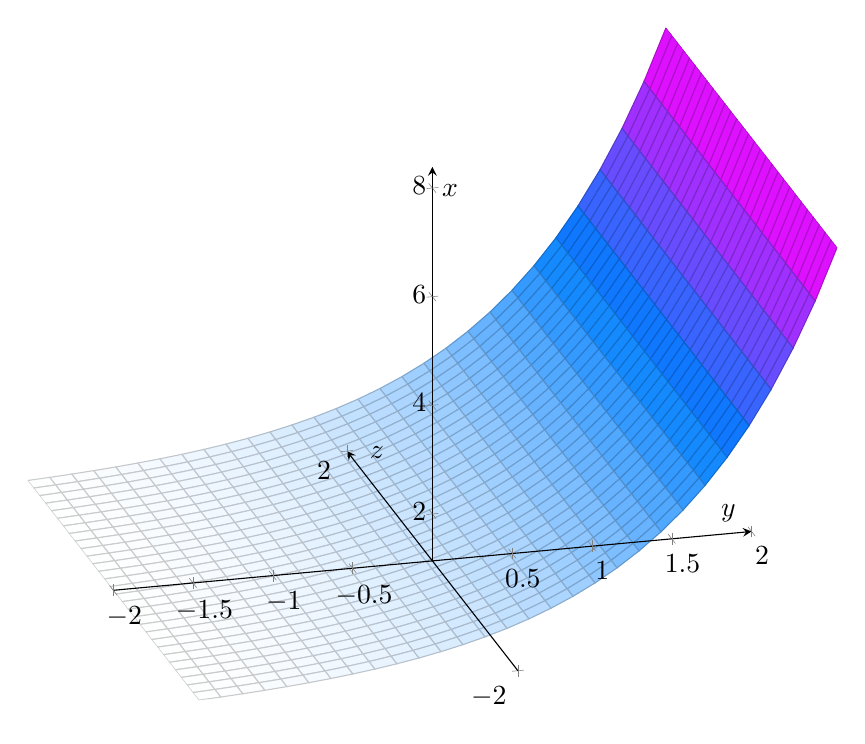
\begin{tikzpicture}
  \begin{axis}[
    view={-15}{30},
    axis lines=center,
    xlabel={$y$},
    ylabel={$z$},
    zlabel={$x$},
    domain=-2:2,
    samples=30,
    colormap/cool,
    mesh/ordering=y varies,
    scale=1.5,
    axis on top,
  ]
    \addplot3[surf]{exp(x)+1};
  \end{axis}
\end{tikzpicture}
\end{center}

\hfill

\noindent (b)
\begin{center}
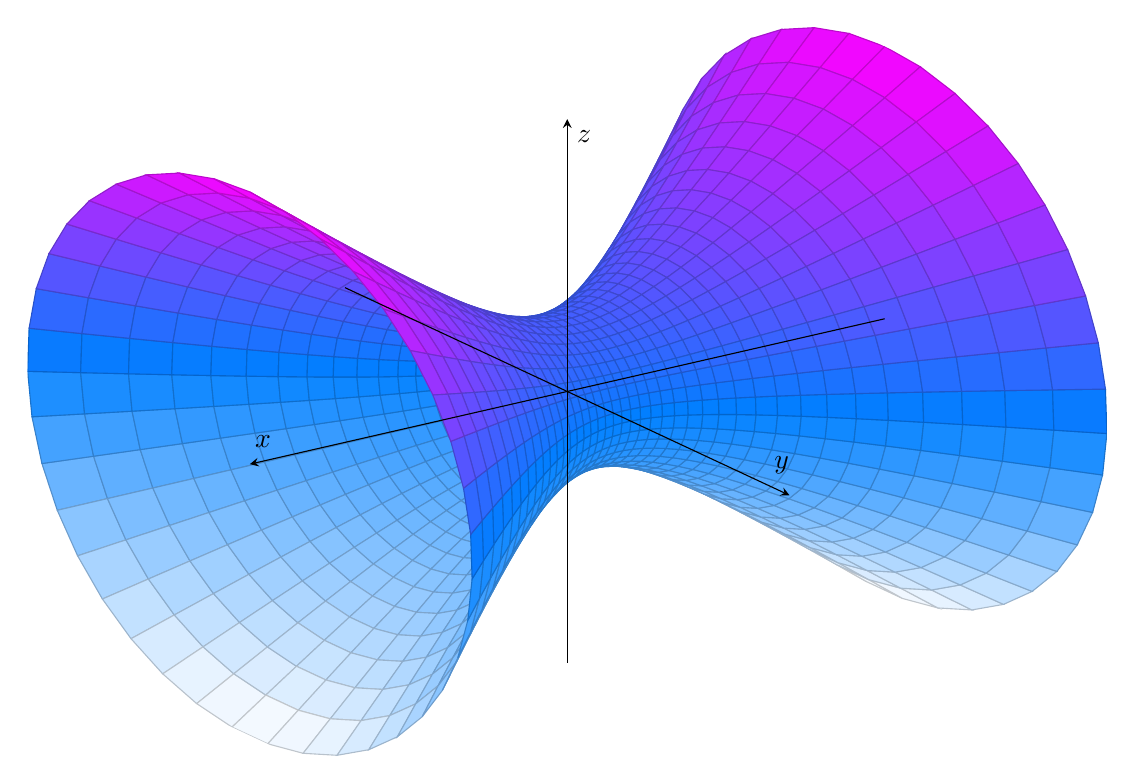
\begin{tikzpicture}
  \begin{axis}[
    view={145}{25},
    xlabel={$x$},
    ylabel={$y$},
    zlabel={$z$},
    axis lines=center,
    domain=0:360,
    y domain=-2:2,
    samples=40,
    axis on top,
    colormap/cool,
    scale=2,
    ticklabel style={anchor=base},
    z buffer=sort, 
    xtick=\empty, ytick=\empty, ztick=\empty,
  ]
  
  \addplot3[surf] ({sinh(y)},{cosh(y)*sin(x)},{cosh(y)*cos(x)});
  \end{axis}
\end{tikzpicture}
\end{center}

\hfill

\noindent 4. Apply the Two Different Paths Test.

\[y=x\implies\lim_{(x,y)\to(0,0)}\frac{x^5y^3}{x^7+y^{21/2}}=\lim_{x\to0}\frac{x^8}{x^7\left(1+x^{7/2}\right)}=\lim_{x\to0}\frac x{1+x^{7/2}}=\frac01=0\]
\[y=x^{2/3}\implies\lim_{(x,y)\to(0,0)}\frac{x^5y^3}{x^7+y^{21/2}}=\lim_{x\to0}\frac{x^7}{2x^7}=\frac12\]

\hfill

\noindent Since $0\neq\dfrac12$, by the Two Different Paths Test, the limit does not exist.

\hfill

\noindent 5. For every $\epsilon>0$, there exists a $\delta>0$ such that

\[0<\sqrt{(x-0)^2+(y-0)^2}<\delta\implies\left|f(x,y)-L\right|<\epsilon\]

\hfill

\noindent The value of the function at $(0,0)$ is $f(0,0)=6\cdot0^2+7\cdot0^2=0$. So, we expect that the limit of the function at this point is $0$.

\[\left|6x^2+7y^2\right|=6x^2+7y^2\qquad\left[x^2\geq0,\quad y^2\geq0\right]\]
\[6x^2+7y^2\leq7x^2+7y^2=7\left(x^2+y^2\right)<7\delta^2\qquad\left[0<\sqrt{x^2+y^2}<\delta\right]\]

\hfill

\noindent Set $\delta=\sqrt{\dfrac\epsilon7}$.

\[\left|f(x,y)-L\right|=|6x^2+7y^2-0|=6x^2+7y^2<7\delta^2=\epsilon\]

\hfill

\noindent Since the limit is the value of the function at this point, $f$ is continuous at $(x,y)=(0,0)$.

\hfill

\noindent 6. $w$ is a function of $x,\:y,\:z$ and $x,\:y,\:z$ are functions of $r,\:s,\:t$. Namely, $w=w(x,y,z),\:x=x(r,s,t),\:y=y(r,s,t),\:z=z(r,s,t)$. Apply the chain rule.

\[\frac{\partial w}{\partial r}=\frac{\partial w}{\partial x}\cdot\frac{\partial x}{\partial r}+\frac{\partial w}{\partial y}\cdot\frac{\partial y}{\partial r}+\frac{\partial w}{\partial z}\cdot\frac{\partial z}{\partial r}\]

\[\frac{\partial w}{\partial x}=\mathrm{e}^{2x-y+3z^2}\cdot2,\quad\frac{\partial w}{\partial y}=\mathrm{e}^{2x-y+3z^2}\cdot(-1),\quad\frac{\partial w}{\partial z}=\mathrm{e}^{2x-y+3z^2}\cdot(6z)\]

\[\frac{\partial x}{\partial r}=1,\quad\frac{\partial y}{\partial r}=2,\quad\frac{\partial z}{\partial r}=-2\sin(rst)\cdot st\]

\[\frac{\partial w}{\partial r}=2\mathrm{e}^{2x-y+3z^2}-2\mathrm{e}^{2x-y+3z^2}-12z\mathrm{e}^{2x-y+3z^2}\sin(rst)st=\boxed{-12zst\cdot\mathrm{e}^{2x-y+3z^2}\cdot\sin(rst)}\]

\hfill

\noindent 7. The volume and the surface area of a right circular cylinder are as follows, respectively.

\[V(D,h)=\frac{\pi D^2h}4,\quad S(D,h)=\pi Dh+\frac{\pi D^2}2,\]

\noindent where $D$ is the diameter of the base and $D=2r$.

\hfill

\noindent (a) The total differential of $V$ is

\[dV=V_D\cdot dD+V_h\cdot dh\]

\hfill

\noindent Calculate the partial derivatives.

\[V_D=\frac{\pi Dh}2,\quad V_h=\frac{\pi D^2}4\]

\hfill

\noindent It is given $\left|dD\right|\leq0.5,\:|dh|\leq0.5,\:D=4,\:h=8$. The bounds for the propagated error in calculating the volume is

\[|dV|\leq\frac{\pi\cdot4\cdot8}2\cdot0.5+\frac{\pi\cdot4^2}4\cdot0.5=8\pi+2\pi=\boxed{10\pi\:\text{cm}^3}\]

\hfill

\noindent (b) The total differential of $S$ is

\[dS=S_D\cdot dD+S_h\cdot dh\]

\hfill

\noindent Calculate the partial derivatives.

\[S_D=\pi h+\pi D,\quad S_h=\pi D\]

\hfill

\noindent It is given $\left|dD\right|\leq0.5,\:|dh|\leq0.5,\:D=4,\:h=8$. The bounds for the propagated error in calculating the surface area is

\[|dS|=\pi\left(8+4\right)\cdot0.5+4\pi\cdot0.5=6\pi+2\pi=\boxed{8\pi\:\text{cm}^2}\]

\hfill

\noindent 8. The normal vector to the surface is $\left\langle0,\ln z,\frac yz+1\right\rangle$. At the point $(1,0,2)$, the normal vector is $\left\langle0,\ln2,1\right\rangle$. The dot product of the normal vector to the surface and the vector that is parallel to the direction of the line is $0$. Let $\mathbf v=\langle 0,b,c\rangle$ be the direction vector of the line. The $x$-component is $0$ because the line is parallel to the $yz$-plane.

\[\langle0,\ln2,1\rangle\cdot\langle0,b,c\rangle=b\ln2+c=\implies \frac cb=-\ln2\]

\hfil

\noindent The slope of the line is $\dfrac{dz}{dy}$ on the $yz$-plane, which is $\dfrac cb$. Therefore, the slope is $\boxed{-\ln2}$.

\hfill

\noindent 9. The equation for the tangent plane to the surface defined by $z=f(x,y)$ at a point $P_0(x_0,y_0,z_0)$ is given by $z-z_0=f_x(x-x_0)+f_y(y-y_0)$.

\[x_0=0,\quad y_0=1,\quad z=3,\quad f_x=\cos x+y\mathrm{e}^{xy},\quad f_y=x\mathrm{e}^{xy}+2\]
\[P=(0,1,3)\quad\rightarrow\quad f_x(0,1)=2,\quad f_y(0,1)=2\]

\hfill

\noindent The equation for the tangent plane is

\[\boxed{z-3=2(x-0)+2(y-1)\implies z=2x+2y+1}\]

\end{document}